\subsection{Pruebas hardware}

\subsubsection{Pruebas de la placa de audio}

Para probar la placa de audio, la colocamos sola, alimentándola con una fuente de alimentación de laboratorio, colocando un Jumper entre el terminal de ADC y DAC para no tener en cuenta el procesado digital.

Después, se introduce una señal sinusoidal y se mide la amplitud de salida, calculando la respuesta en frecuencia del circuito. Se recoge una gráfica con la respuesta en frecuencia en decibelios relativos al máximo en la \autoref{fig:4-2-1-respuesta-cascos} (auriculares) y la \autoref{fig:4-2-1-respuesta-altavoces} (altavoces). Cabe destacar que la respuesta dibujada es en decibelios relativos al máximo, por lo que parece que tienen la misma amplitud, pero el altavoz duplica la amplitud de la señal de entrada.

\begin{figure}[h]
    \centering
    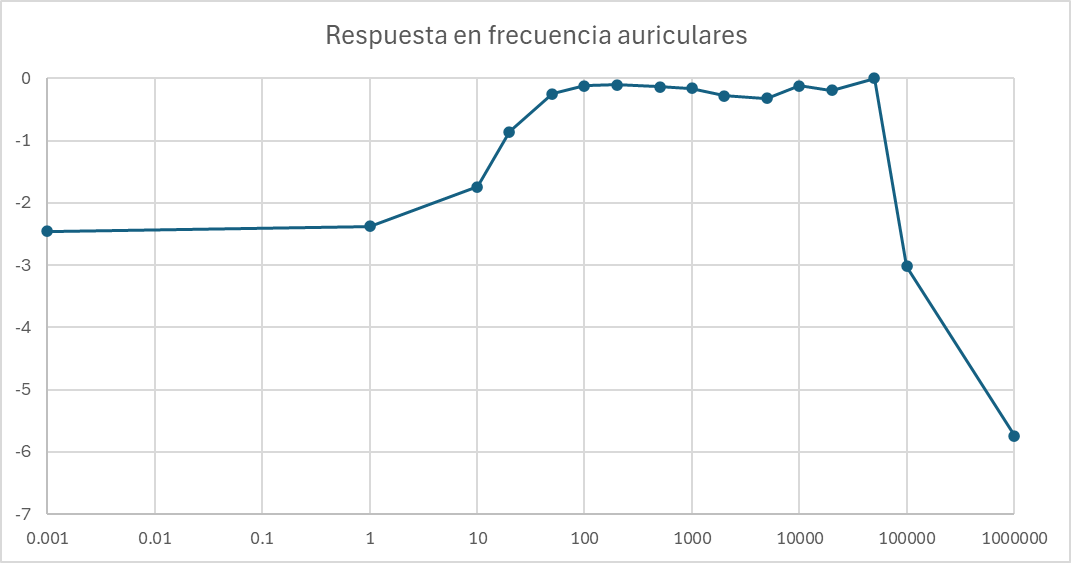
\includegraphics[width=0.5\textwidth]{images/4/4-2/respuesta-auriculares.png}
    \caption{Respuesta del circuito amplificador de auriculares}
    \label{fig:4-2-1-respuesta-cascos}
\end{figure}

\begin{figure}[h]
    \centering
    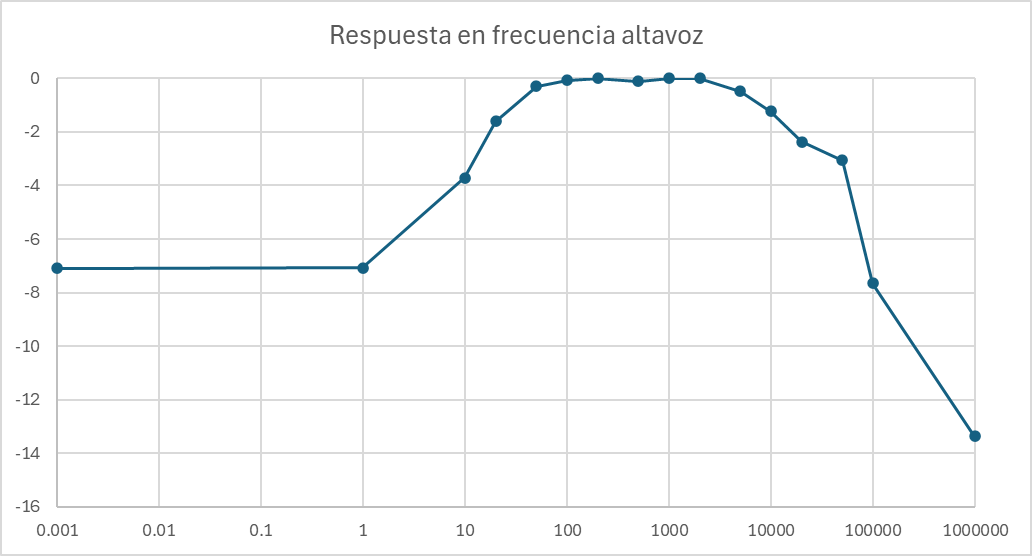
\includegraphics[width=0.5\textwidth]{images/4/4-2/respuesta-altavoces.png}
    \caption{Respuesta del circuito amplificador de altavoces}
    \label{fig:4-2-1-respuesta-altavoces}
\end{figure}

Comprobando el circuito de habilitación, funciona adecuadamente pero a veces se comporta de forma poco consistente al intentar desactivar el circuito cuando está habitado, pero generalmente se comporta correctamente. 

Por otro lado, conectamos distintas cargas y medimos el consumo del circuito, obteniendo los siguientes valores de consumo en función de la impedancia nominal del altavoz. Obtenemos los siguientes valores:
\begin{enumerate}
    \item Auriculates de $~40\ \Omega$: Consumo de $4\ mA$
    \item Altavoz de $8\ \Omega$: Consumo $64\ mA$
    \item Altavoz de $4\ \Omega$: Consumo de $164\ mA$
\end{enumerate}

Además, probando el cambiador de nivel, vemos que consigue una tensión de nivel bajo de $19.78\ mV$ y un $6.99\ V$.

\subsubsection{Pruebas del circuito de alimentación}

Para realizas las pruebas del circuito de alimentación, probamos primero a realizar una descarga y carga de la batería para probar este funcionamiento. Descargamos la batería hasta un valor aproximado de $3.5\ V$ y la volvimos a cargar con nuestro cargador hasta un valor de $4.05\ V$, en el cual la corriente de carga comienza a disminuir y el proceso de carga se ralentiza.

En condiciones normales, la batería carga con una corriente constante de entre $600$ y $700\ mA$, pero disminuye en el tramo final como se comentó en el diseño del circuito. También se ha probado a cargar el circuito a la vez que se carga la batería. Si la fuente tiene suficiente capacidad como para alimentar las dos cosas, hemos comprobado que así lo hace. Hemos probado por ejemplo con una carga de $10\ \Omega$, con lo que el consumo de aproximadamente $
700\ mA$ se suma a la carga obteniendo cerca de $1.5\ A$.

Por otro lado, caracterizamos la regulación de carga para comprobar que nuestro circuito mantuviera la tensión de salida incluso cuando es demandado una gran cantidad de corriente. Se ve que obtenemos un valor de $-39.012 V/A$, o $0.56\%/A$, un buen valor contando con que el consumo aproximado será de medio amperio. Se recoge la gráfica de las medidas en la \autoref{fig:4-2-2-regulacion-carga}.

\begin{figure}[h]
    \centering
    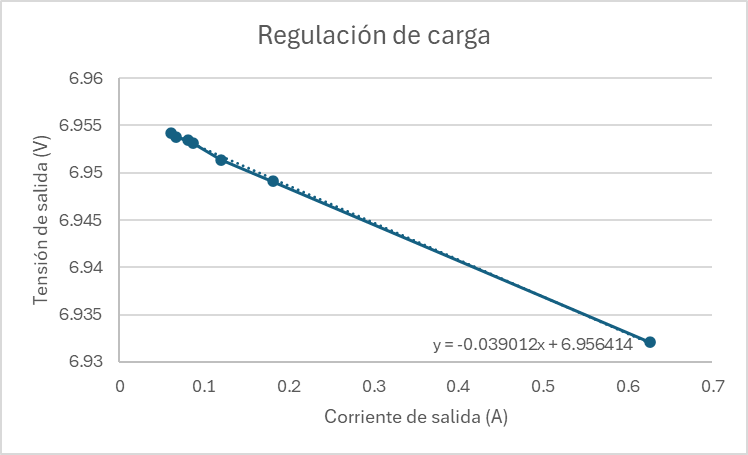
\includegraphics[width=0.5\textwidth]{images/4/4-2/regulacion-carga.png}
    \caption{Regulación de carga del circuito de baterías}
    \label{fig:4-2-2-regulacion-carga}
\end{figure}

Además, comprobamos que los indicadores luminosos funcionan correctamente ya que se enciende el verde cuando se conecta la alimentación y el rojo cuando se está cargando la batería. Al finalizar la carga, se apaga la luz roja y si se enchufa sin estar conectada parpadea el indicador rojo.

Mediante el osciloscopio medimos la tensión de salida del circuito de alimentación, observando que presenta un ruido en muy alta frecuencia, como se puede ver en la \autoref{fig:4-2-2-ruido}. Creemos que este pico de ruido es el culpable de la inestabilidad de los relojes de la placa, pero al colocar condensadores en paralelo no conseguimos reducirlo.

\begin{figure}[h]
    \centering
    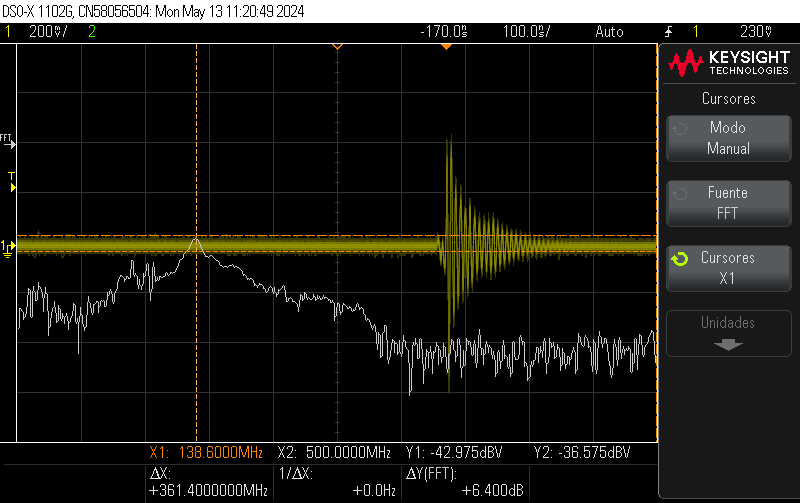
\includegraphics[width=0.5\textwidth]{images/4/4-2/ruido.png}
    \caption{Ruido en la señal de alimentación}
    \label{fig:4-2-2-ruido}
\end{figure}